% ******************************* PhD Thesis Template **************************
% Please have a look at the README.md file for info on how to use the template

\documentclass[a4paper,12pt,times,numbered,print,index]{Classes/PhDThesisPSnPDF}

\RequirePackage[utf8]{inputenc}
\DeclareMathOperator*{\argmax}{argmax}
\DeclareMathOperator*{\argmin}{argmin}
\DeclareMathOperator*{\simm}{sim}

% ******************************************************************************
% ******************************* Class Options ********************************
% *********************** See README for more details **************************
% ******************************************************************************

% `a4paper'(The University of Cambridge PhD thesis guidelines recommends a page
% size a4 - default option) or `a5paper': A5 Paper size is also allowed as per
% the Cambridge University Engineering Department guidelines for PhD thesis
%
% `11pt' or `12pt'(default): Font Size 10pt is NOT recommended by the University
% guidelines
%
% `oneside' or `twoside'(default): Printing double side (twoside) or single
% side.
%
% `print': Use `print' for print version with appropriate margins and page
% layout. Leaving the options field blank will activate Online version.
%
% `index': For index at the end of the thesis
%
% `draftclassic': For draft mode without loading any images (same as draft in book)
%
% `draft': Special draft mode with line numbers, images, and water mark with
% timestamp and custom text. Position of the text can also be modified.
%
% `abstract': To generate only the title page and abstract page with
% dissertation title and name, to submit to the Student Registry
%
% `chapter`: This option enables only the specified chapter and it's references
%  Useful for review and corrections.
%
% ************************* Custom Page Margins ********************************
%
% `custommargin`: Use `custommargin' in options to activate custom page margins,
% which can be defined in the preamble.tex. Custom margin will override
% print/online margin setup.
%
% *********************** Choosing the Fonts in Class Options ******************
%
% `times' : Times font with math support. (The Cambridge University guidelines
% recommend using times)
%
% `fourier': Utopia Font with Fourier Math font (Font has to be installed)
%            It's a free font.
%
% `customfont': Use `customfont' option in the document class and load the
% package in the preamble.tex
%
% default or leave empty: `Latin Modern' font will be loaded.
%
% ********************** Choosing the Bibliography style ***********************
%
% `authoryear': For author-year citation eg., Krishna (2013)
%
% `numbered': (Default Option) For numbered and sorted citation e.g., [1,5,2]
%
% `custombib': Define your own bibliography style in the `preamble.tex' file.
%              `\RequirePackage[square, sort, numbers, authoryear]{natbib}'.
%              This can be also used to load biblatex instead of natbib
%              (See Preamble)
%
% **************************** Choosing the Page Style *************************
%
% `default (leave empty)': For Page Numbers in Header (Left Even, Right Odd) and
% Chapter Name in Header (Right Even) and Section Name (Left Odd). Blank Footer.
%
% `PageStyleI': Chapter Name next & Page Number on Even Side (Left Even).
% Section Name & Page Number in Header on Odd Side (Right Odd). Footer is empty.
%
% `PageStyleII': Chapter Name on Even Side (Left Even) in Header. Section Number
% and Section Name in Header on Odd Side (Right Odd). Page numbering in footer

% Uncomment to change page style
%\pagestyle{PageStyleII}

% ********************************** Preamble **********************************
% Preamble: Contains packages and user-defined commands and settings
% ******************************************************************************
% ****************************** Custom Margin *********************************

% Add `custommargin' in the document class options to use this section
% Set {innerside margin / outerside margin / topmargin / bottom margin}  and
% other page dimensions
\ifsetCustomMargin
    \RequirePackage[left=37mm,right=30mm,top=35mm,bottom=30mm]{geometry}
    \setFancyHdr % To apply fancy header after geometry package is loaded
\fi

% Add spaces between paragraphs
%\setlength{\parskip}{0.5em}
% Ragged bottom avoids extra whitespaces between paragraphs
\raggedbottom
% To remove the excess top spacing for enumeration, list and description
%\usepackage{enumitem}
%\setlist[enumerate,itemize,description]{topsep=0em}

% *****************************************************************************
% ******************* Fonts (like different typewriter fonts etc.)*************

% Add `customfont' in the document class option to use this section

\ifsetCustomFont
    % Set your custom font here and use `customfont' in options. Leave empty to
    % load computer modern font (default LaTeX font).
    %\RequirePackage{helvet}

    % For use with XeLaTeX
    %  \setmainfont[
    %    Path              = ./libertine/opentype/,
    %    Extension         = .otf,
    %    UprightFont = LinLibertine_R,
    %    BoldFont = LinLibertine_RZ, % Linux Libertine O Regular Semibold
    %    ItalicFont = LinLibertine_RI,
    %    BoldItalicFont = LinLibertine_RZI, % Linux Libertine O Regular Semibold Italic
    %  ]
    %  {libertine}
    %  % load font from system font
    %  \newfontfamily\libertinesystemfont{Linux Libertine O}
\fi

% *****************************************************************************
% **************************** Custom Packages ********************************

% ************************* Algorithms and Pseudocode **************************
\usepackage{algorithm2e}
\usepackage{listings}
\usepackage{algpseudocode}


% ********************Captions and Hyperreferencing / URL **********************

% Captions: This makes captions of figures use a boldfaced small font.
%\RequirePackage[small,bf]{caption}

\RequirePackage[labelsep=space,tableposition=top]{caption}
\renewcommand{\figurename}{Fig.} %to support older versions of captions.sty


% *************************** Graphics and figures *****************************

%\usepackage{rotating}
%\usepackage{wrapfig}

% Uncomment the following two lines to force Latex to place the figure.
% Use [H] when including graphics. Note 'H' instead of 'h'
\usepackage{float}
\restylefloat{figure}

% Subcaption package is also available in the sty folder you can use that by
% uncommenting the following line
% This is for people stuck with older versions of texlive
%\usepackage{sty/caption/subcaption}
\usepackage{subcaption}

% ********************************** Tables ************************************
\usepackage{booktabs} % For professional looking tables
\usepackage{multirow}

%\usepackage{multicol}
%\usepackage{longtable}
%\usepackage{tabularx}


% *********************************** SI Units *********************************
\usepackage{siunitx} % use this package module for SI units


% ******************************* Line Spacing *********************************

% Choose linespacing as appropriate. Default is one-half line spacing as per the
% University guidelines

% \doublespacing
% \onehalfspacing
% \singlespacing


% ************************ Formatting / Footnote *******************************
\usepackage{blindtext}
\usepackage{amsmath}
\usepackage{booktabs}
\usepackage{graphicx}
\RestyleAlgo{algoruled}

% Don't break enumeration (etc.) across pages in an ugly manner (default 10000)
%\clubpenalty=500
%\widowpenalty=500
%\usepackage[perpage]{footmisc} %Range of footnote options


% *****************************************************************************
% *************************** Bibliography  and References ********************

%\usepackage{cleveref} %Referencing without need to explicitly state fig /table

% Add `custombib' in the document class option to use this section
\ifuseCustomBib
    % \RequirePackage[square, sort, numbers, authoryear]{natbib} % CustomBib

    % If you would like to use biblatex for your reference management, as opposed to the default `natbibpackage` pass the option `custombib` in the document cl`ass. Comment out the previous line to make sure you don't load the natbib package. Uncomment the following lines and specify the location of references.bib file

    % \RequirePackage[backend=biber, style=numeric-comp, citestyle=numeric, sorting=nty, natbib=true]{biblatex}
    \addbibresource{References/references.bib} %Location of references.bib only for biblatex, Do not omit the .bib extension from the filename.

\fi

% changes the default name `Bibliography` -> `References'
\renewcommand{\bibname}{References}


% ******************************************************************************
% ************************* User Defined Commands ******************************
% ******************************************************************************

% *********** To change the name of Table of Contents / LOF and LOT ************

%\renewcommand{\contentsname}{My Table of Contents}
%\renewcommand{\listfigurename}{My List of Figures}
%\renewcommand{\listtablename}{My List of Tables}


% ********************** TOC depth and numbering depth *************************

\setcounter{secnumdepth}{2}
\setcounter{tocdepth}{2}


% ******************************* Nomenclature *********************************

% To change the name of the Nomenclature section, uncomment the following line

%\renewcommand{\nomname}{Symbols}


% ********************************* Appendix ***********************************

% The default value of both \appendixtocname and \appendixpagename is `Appendices'. These names can all be changed via:

%\renewcommand{\appendixtocname}{List of appendices}
%\renewcommand{\appendixname}{Appndx}

% *********************** Configure Draft Mode **********************************

% Uncomment to disable figures in `draft'
%\setkeys{Gin}{draft=true}  % set draft to false to enable figures in `draft'

% These options are active only during the draft mode
% Default text is "Draft"
%\SetDraftText{DRAFT}

% Default Watermark location is top. Location (top/bottom)
%\SetDraftWMPosition{bottom}

% Draft Version - default is v1.0
%\SetDraftVersion{v1.1}

% Draft Text grayscale value (should be between 0-black and 1-white)
% Default value is 0.75
%\SetDraftGrayScale{0.8}


% ******************************** Todo Notes **********************************
%% Uncomment the following lines to have todonotes.

%\ifsetDraft
%	\usepackage[colorinlistoftodos]{todonotes}
%	\newcommand{\mynote}[1]{\todo[author=kks32,size=\small,inline,color=green!40]{#1}}
%\else
%	\newcommand{\mynote}[1]{}
%	\newcommand{\listoftodos}{}
%\fi

% Example todo: \mynote{Hey! I have a note}

% *****************************************************************************
% ******************* Better enumeration my MB*************
\usepackage{enumitem}



% ************************ Thesis Information & Meta-data **********************
% Thesis title and author information, refernce file for biblatex
% ************************ Thesis Information & Meta-data **********************
%% The title of the thesis
\title{Repurposing Drugs for the Rapid Response to Epidemics and Pandemics}
%\texorpdfstring is used for PDF metadata. Usage:
%\texorpdfstring{LaTeX_Version}{PDF Version (non-latex)} eg.,
%\texorpdfstring{$sigma$}{sigma}

%% Subtitle (Optional)
\subtitle{Using Batch Active Learning}

%% The full name of the author
\author{Ross Brown}

%% Department (eg. Department of Engineering, Maths, Physics)
\dept{Department of Chemical Engineering and Biotechnology}

%% University and Crest
\university{University of Cambridge}
% Crest minimum should be 30mm.
\crest{
\includegraphics[width=0.2\textwidth]{University_Crest}}
%% Use this crest, if you are using the college crest
%% Crest long miminum should be 65mm
%\crest{
\includegraphics[width=0.45\textwidth]{University_Crest_Long}}

%% College shield [optional] 
% Crest minimum should be 30mm.
%\collegeshield{
\includegraphics[width=0.2\textwidth]{CollegeShields/Kings}}


%% Supervisor (optional)
%% for multiple supervisors, append each supervisor with the \newline command
%\supervisor{Prof. A.B. Supervisor\newline
%Prof. C.D. Supervisor}

%% Supervisor Role (optional) - Supervisor (default) or advisor
% \supervisorrole{\textbf{Supervisors: }}
%% if no title is desired:
% \supervisorrole{}

%% Supervisor line width: required to align supervisors
%\supervisorlinewidth{0.35\textwidth}

%% Advisor (optional)
%% for multiple advisors, append each advisor with the \newline command
%\advisor{Dr. A. Advisor\newline
%Dr. B. Advisor}

%% Advisor Role (optional) - Advisor (default) or leave empty
% \advisorrole{Advisors: }
%% if no title is required
% \advisorrole{}

%% Advisor line width: required to align supervisors
%\advisorlinewidth{0.25\textwidth}


%% You can redefine the submission text:
% Default as per the University guidelines:
% ``This dissertation is submitted for the degree of''
%\renewcommand{\submissiontext}{change the default text here if needed}

%% Full title of the Degree
\degreetitle{Master of Engineering}

%% College affiliation (optional)
\college{Robinson College}

%% Submission date
% Default is set as {\monthname[\the\month]\space\the\year}
%\degreedate{September 2014} 

%% Meta information
\subject{Masters Thesis} \keywords{{LaTeX} {Masters Thesis} {Chemical Engineering} {University of Cambridge} {Machine Learning} {Drug Discovery}}


% ***************************** Abstract Separate ******************************
% To printout only the titlepage and the abstract with the PhD title and the
% author name for submission to the Student Registry, use the `abstract' option in
% the document class.

\ifdefineAbstract
 \pagestyle{empty}
 \includeonly{Declaration/declaration, Abstract/abstract}
\fi

% ***************************** Chapter Mode ***********************************
% The chapter mode allows user to only print particular chapters with references
% Title, Contents, Frontmatter are disabled by default
% Useful option to review a particular chapter or to send it to supervisior.
% To use choose `chapter' option in the document class

\ifdefineChapter
 \includeonly{Chapter3/chapter3}
\fi

% ******************************** Front Matter ********************************
\begin{document}

\frontmatter

\maketitle

% ******************************* Thesis Dedidcation ********************************

\begin{dedication}

    I would like to dedicate this thesis to the loss of sleep never to be recovered. It's sacrifice in making this project come to fruition will never be forgotten.

\end{dedication}


% ******************************* Thesis Declaration ***************************

\begin{declaration}

I hereby declare that except where specific reference is made to the work of 
others, the contents of this dissertation are original and have not been 
submitted in whole or in part for consideration for any other degree or 
qualification in this, or any other university. This dissertation is my own 
work and contains nothing which is the outcome of work done in collaboration 
with others, except as specified in the text and Acknowledgements. This 
dissertation contains fewer than 65,000 words including appendices, 
bibliography, footnotes, tables and equations and has fewer than 150 figures.

% Author and date will be inserted automatically from thesis.tex \author \degreedate

\end{declaration}


% % ************************** Thesis Acknowledgements **************************

\begin{acknowledgements}      


And I would like to acknowledge ...


\end{acknowledgements}

% ************************** Thesis Abstract *****************************
% Use `abstract' as an option in the document class to print only the titlepage and the abstract.



\begin{abstract}

  The SARS-CoV-2 pandemic saw a high death toll which was reduced as drugs such as Remdesivir were introduced as treatments. This process was slow and few drugs were found capable of reducing the mortality of the virus. A solution to this issue is presented: finding existing, workable treatments using batch active learning. This combines greedy methodologies with clusters and uncertainty analysis, accumulating in a final algorithm \textit{RoDGer}. Algorithms were compared with each other, with the final algorithm learning the datasets at a 10\% faster rate than simply randomly sampling.

\end{abstract}


% *********************** Adding TOC and List of Figures ***********************

\tableofcontents

% \listoffigures

% \listoftables

% \printnomenclature[space] space can be set as 2em between symbol and description
\printnomenclature[5em]

%\printnomenclature

% ******************************** Main Matter *********************************
\mainmatter
%!TEX root = ../thesis.tex
%*******************************************************************************
%*********************************** First Chapter *****************************
%*******************************************************************************

\chapter{Introduction}  %Title of the First Chapter

\ifpdf
    \graphicspath{{Chapter1/Figs/Raster/}{Chapter1/Figs/PDF/}{Chapter1/Figs/}}
\else
    \graphicspath{{Chapter1/Figs/Vector/}{Chapter1/Figs/}}
\fi

In 2019, human civilisation was on the precipice of a natural disaster: \mbox{SARS-CoV-2} (\mbox{COVID-19}). First reported to the World Health Organization (WHO) on December 31st, it became officially recognised as a pandemic on March 11th 2020. As of the writing of this passage, 515 million cases and 18 million excess deaths have been recorded \cite{Wan22,WHO22}. This, however, is not the first time a pandemic has occurred, with the Black Death infamously killing a third of Europe's population and the Spanish Flu causing mass death throughout the world. Likewise, it is unlikely to be the last.

When such a disaster does strike, it is important to react quickly. Vaccinations are developed and manufactured on accelerated timelines, cutting development time from years to months. Trials into potential treatments are encouraged with haste. When speed is not achieved with these measures, misinformation rapidly spreads. Within the first stages of the pandemic, drugs such as hydroxychloroquine and bleach were amongst several that were promoted by the President of the United States of America demonstrating the desperation in finding therapeutic drugs against the virus.

In order to facilitate a more robust approach to finding treatments, the FDA instigated the Coronavirus Treatment Acceleration Program (CTAP) \cite{CTAP22}. Here, over 690 drugs are in the development stage with over 450 clinical trials underway to investigate the effectiveness, with 15 drugs currently authorised for emergency use and only one drug, remdesivir, with approval for use against \mbox{COVID-19} \cite{CTAP22}. These results, and the timescale in which they were achieved, is suboptimal. This is due to the slow, labourous, methods used in investigations into pre-existing drugs slow. Flawed selection priorities due to an information overload on scientists. This resulted in delays in treatment. Time many did not have.

A hopeful fulfilment of this problem is the "Robot Scientist" \cite{And10}; a fully automated combination of software and hardware aimed at solving this problem. For the software side, a form of reinforcement machine learning is proposed: batch active learning. This is a methodology suited to fields with large amounts of unlabelled data which is difficult to label. In this case, the labelling requires chemical and biological experimentation costing both time and money. By using active learning, as few drugs as possible will be labelled within this stage to accurately predict the best drugs for the given problem. From here, accelerated, targetted clinical trials may begin.

Due to the large importance of time, many drugs may be tested in parallel. This becomes even more practically considering the eistence of robotic testing fascilities. This presents an additional problem: how does one set up a testing scheme for batches? Can the same techniques used in single site learning be transitioned across, or are more inventive methodogies required here?

Thus, the purpose of this thesis. To present an algorithm which may be used to discover effective drugs within a short period of time. Additionally, a framework will be developed that allows for different algorithms to be rigorously compared to each other for increased robustness.
%!TEX root = ../thesis.tex
%*******************************************************************************
%****************************** Second Chapter *********************************
%*******************************************************************************

\chapter{Previous Work}
\label{ch:2}

\graphicspath{{Chapter2/Figs/Vector/}{Chapter2/Figs/Raster/}}

% **************************** Nomenclature **********************************
\nomenclature[c-1-x]{$x$}{Data points where $x=\{x_0, x_1, ..., x_{N-1}\}$}
\nomenclature[c-1-y]{$y$}{Labels for the dataset where $y=\{y_0, y_1, ..., y_{N-1}\}$}
\nomenclature[c-1-N]{$N$}{Number of features (dimensions) of $x$}

\nomenclature[c-1-s]{$s_g$}{Sample standard deviation of the predictions}


\nomenclature[c-2-IC50]{$\mathrm{IC_{50}}$}{Half maximal inhibitory molar concentration}
\nomenclature[c-2-XC50]{$\mathrm{XC_{50}}$}{Half maximal effective or inhibitory molar concentration}
\nomenclature[c-2-EC50]{$\mathrm{EC_{50}}$}{Half maximal effective molar concentration}
\nomenclature[c-2-AC50]{$\mathrm{AC_{50}}$}{Half maximal effective molar concentration}
\nomenclature[c-2-Ki]{$\mathrm{Ki}$}{Half maximal molar concentration for half receptor occupancy}
\nomenclature[c-2-LD50]{$\mathrm{LD_{50}}$}{Median lethal dose}


%*****************************************************************************

In order to assist the understanding of the methodologies used by others within the field of active learning, a toy dataset has been created. It is based upon~(\ref{eq:phantom}) and has been shown in Figure~\ref{fig:phantom}. The $y$ values used within the algorithms have been combined with errors, $\epsilon{}\sim{}\mathcal{N}(0, 0.01)$.

\begin{equation}
    y = \sin{(x_0)}^{10} + \cos{(10 + x_0 x_1)}\cos{(x_0)}
    \label{eq:phantom}
\end{equation}

\begin{figure}[h]
    \begin{center}
        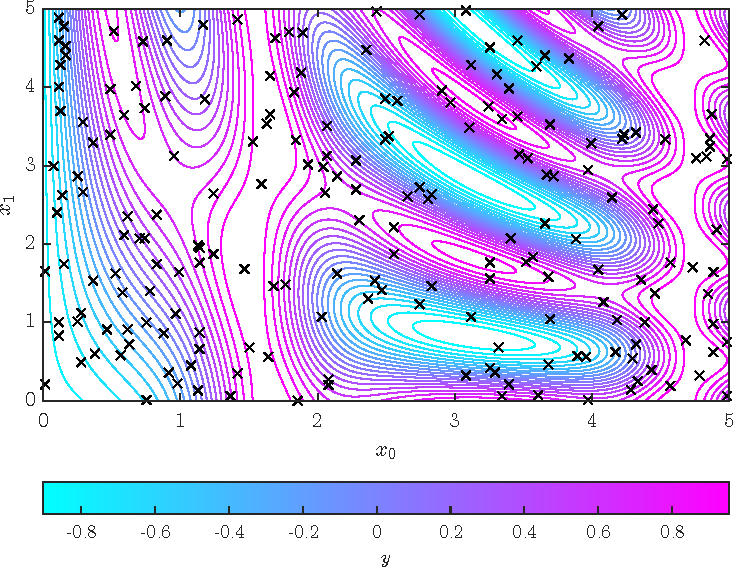
\includegraphics{phantomOverview.pdf}
        \caption[Example Dataset for Representation of Ideas]{Contour plot of the function used to demonstrate the algorithms presented in previous work. The crosses have been used to show the location of the 200 test data points used within this example.}
        \label{fig:phantom}
    \end{center}
\end{figure}

In order to assess the algorithms, the mean squared error (mse) has been used. Comparisons are made to the naive approach of random sampling, i.e. Monte Carlo sampling. Each algorithm will be given five random starting points, and attempted improvement will follow.

\section{Active Learning}
\label{ch:Active Learning}

There are several schools of thought regarding active learning. These can be separated into two distinct categories: current data and future predictions. The former of these is computationally cheaper, more complex t implement, and less adaptable to model changes, as will be apparent on description.

\subsection{Current Data}
\subsubsection{Uncertainty Sampling and Regions of Disagreements}
\label{sec:UncertaintySampling}

The simplest is applicable to cases in which a certainty is provided with each prediction. \textcite{Set09} suggests selecting the data point with the largest uncertainty according to the current model. This has been shown with the toy dataset, as demonstrated in Figure~\ref{fig:rodPhantom}.


\begin{figure}
    \begin{center}
        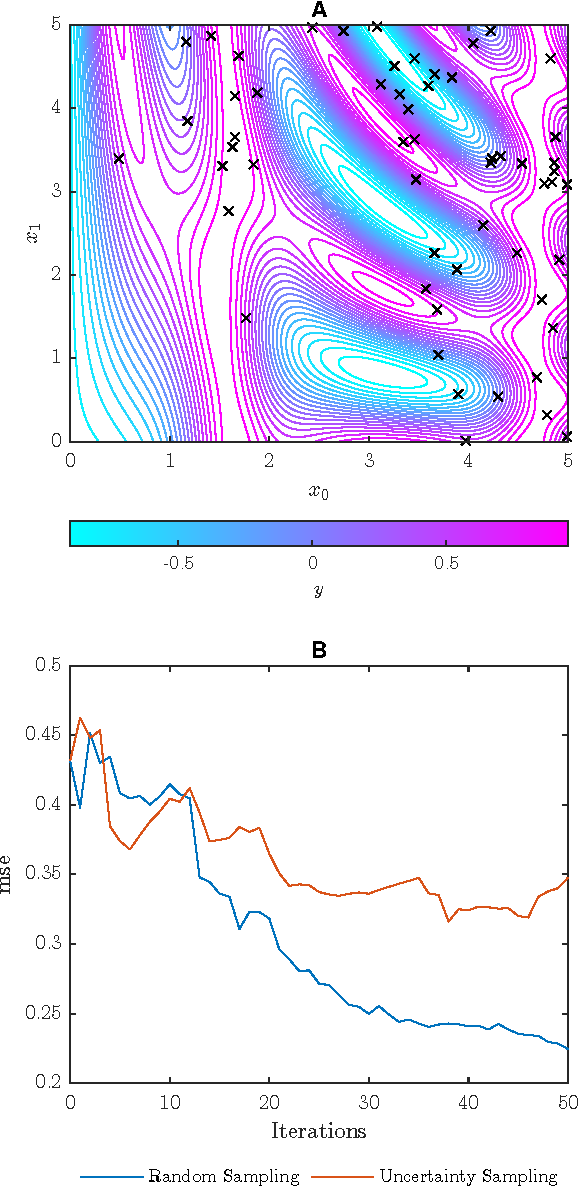
\includegraphics{rodPhantom.pdf}
        \caption[Uncertainty Sampling Demonstration]{The outcome of the investigating the areas of the highest uncertainty. An initial set of 5 random points was provided, and 50 further iterations were then carried out of sample size 1. A) Demonstrates the final set of points tested by the algorithm and B) shows the change in the mean squared error for the algorithm after each iteration.}
        \label{fig:rodPhantom}
    \end{center}
\end{figure}

Interestingly, Figure \ref{fig:rodPhantom}B shows how the mean squared error for the random sampling method performed to worse within the iterations tested. This is likely due to a bias in the use of linear models in fitting leading to large uncertainties surrounding areas with high curvature. Evidence to this is provided in Figure~\ref{fig:rodPhantom}A with a large proportion of the sampled points at areas of high curvature.

\begin{equation}
    \label{eq:x_next1}
    x_\mathrm{next}=\argmax_X{\left[s_{g(X)}\right]}
\end{equation}

As addressed by \textcite{Set09}, this can be extended to any probabilistic model through (\ref{eq:x_next1}). \textcite{Set09} also notes the use of information theory for probabilistic models(\ref{eq:info_uncertainty}), where $y^{*}=\argmax_y{}P(y|x;\theta{})$ is the most likely $y$ for $x$. This derives from the principle that the greatest entropy requires the most information to encode, and thus the least certain. However, \textcite{Set09} fails to address non-probabilistic models in this instance, instead converting such models into probabilistic ones.


\begin{equation}
    \label{eq:info_uncertainty}
    {x_\mathrm{next}=\argmax_X{\left[P(y^{*}|x;\theta{})\right]}}
\end{equation}

In order to adapt non-probabilistic models into probabilistic ones, composite models may be used. These are an amalgamation of other models where the standard deviation of the individual models can be taken as the degree of certainty for a given point. This is commonly referred to minimising the region of disagreement, referring the spaces of discord within the hypothesis space. By minimising the region of disagreement between various models, a more coherent hypothesis space is sought leading to a more accurate model. Indeed, this was the method used in Figure \ref{fig:rodPhantom}. Mathematically, a set of $n$ models ${M = \{m_0,\ldots{}, m_{n-1}\}}$, with each model offering a prediction of $\hat{m_i}$, ${\hat{M}=\frac{1}{n}\sum{\hat{m_i}}}$, and the sample standard deviation of $\hat{m}$ giving the uncertainty.


\textcite{Set09} suggests  third way of interpreting uncertinty. By taking the approach from information theory, (\ref{eq:infoUncert}) is settled upon. This directly states gives the point of the highest entropy, suggesting by knowing the point provides the largest information gain. Notably however, this is difficult to implement with most models, as a probability distribution is required. This could be made simpler by approximating to a normal distribution.

\begin{equation}
    \label{eq:infoUncert}
    x_\mathrm{next}=\argmax_x{\left[\phi_A(x)\times{\left(\frac{1}{U}\sum{\simm{(x, x_i)}}\right)}^\beta\right]}
\end{equation}


% \subsubsection{Broad Knowledge Base}
% A second form stems from information theory. Here, the aim is to produce an evenly dispersed $x$ allowing a well-informed knowledge base. This prevents poor model choice from influencing the algorithm as was seen in \ref{fig:rodPhantom}. There are two paths to proceed: density and nearest neighbours.


% The former of these requires a definition of density in a sparsely populated space. As an analogy, although the density of a gas appears well-defined, it becomes non-smooth once the volume defined over is comparable to the distance between particles. Thus, a new definition is required.

% Alternatively, nearest neighbour requires little explanation. $x_\mathrm{next}$ is the unlabelled data point furthest from any labelled data point. The results of \ref{eq:inverseSim} can be seen in Figure~\ref{fig:b}.

% \begin{equation}
%   \label{eq:inverseSim}
%   x_\mathrm{next}=\argmax_x{\left(\sum{\frac{1}{\simm{(x, x_i)}}}\right)}
% \end{equation}

% \begin{figure}[h]
%   \begin{center}
%     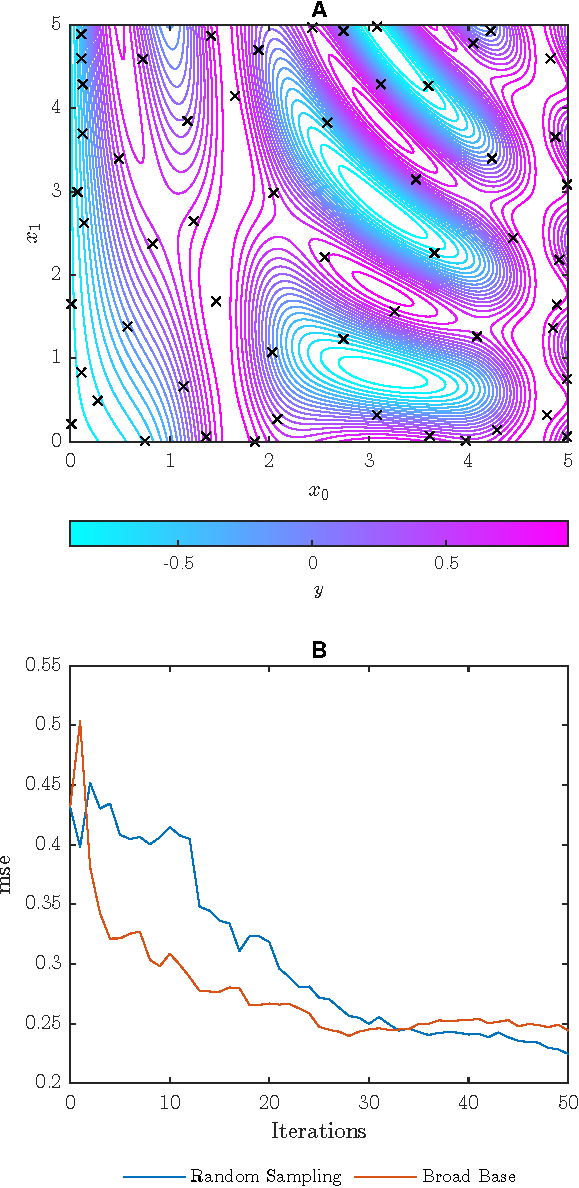
\includegraphics{broadPhantom.pdf}
%     \caption[Broad-Base Sampling Illustration]{The outcome of the investigating the areas of using a broad base. An initial set of 5 random points was provided, and 50 further iterations were then carried out of sample size 1. A) Demonstrates the final set of points tested by the algorithm and B) shows the change in the mean squared error for the algorithm after each iteration.}
%     \label{fig:b}
%   \end{center}
% \end{figure}


\subsubsection{Density Hotspots}
\label{sec:litRevDH}
Conversely, a density weighted model has been suggested, as it escapes the introduction of error from outliers (i.e.\ data points far away from alternative data points). \textcite{Set08} suggest (\ref{eq:Settles_density}) which can be broken down into two parts: a function for selection, $\phi_A$, and a function for similarity, $\simm$. The former arises from  another method described in this section. The latter requires a function to describe the similarity between data points.

\begin{equation}
    \label{eq:Settles_density}
    x_\mathrm{next}=\argmax_x{\left[\phi_A(x)\times{\left(\frac{1}{U}\sum{\simm{(x, x_i)}}\right)}^\beta\right]}
\end{equation}

\textcite{Set08} admit that $\simm$ is open for interpretation. It must also be recognised that this lays the foundation of a clusterisation algorithm. There exist many forms of these algorithms, with the results of several of these algorithms on toy data sets presented in Figure~\ref{fig:ClusterResults} \cite{SciClus}.

\begin{figure}[H]
    \begin{center}
        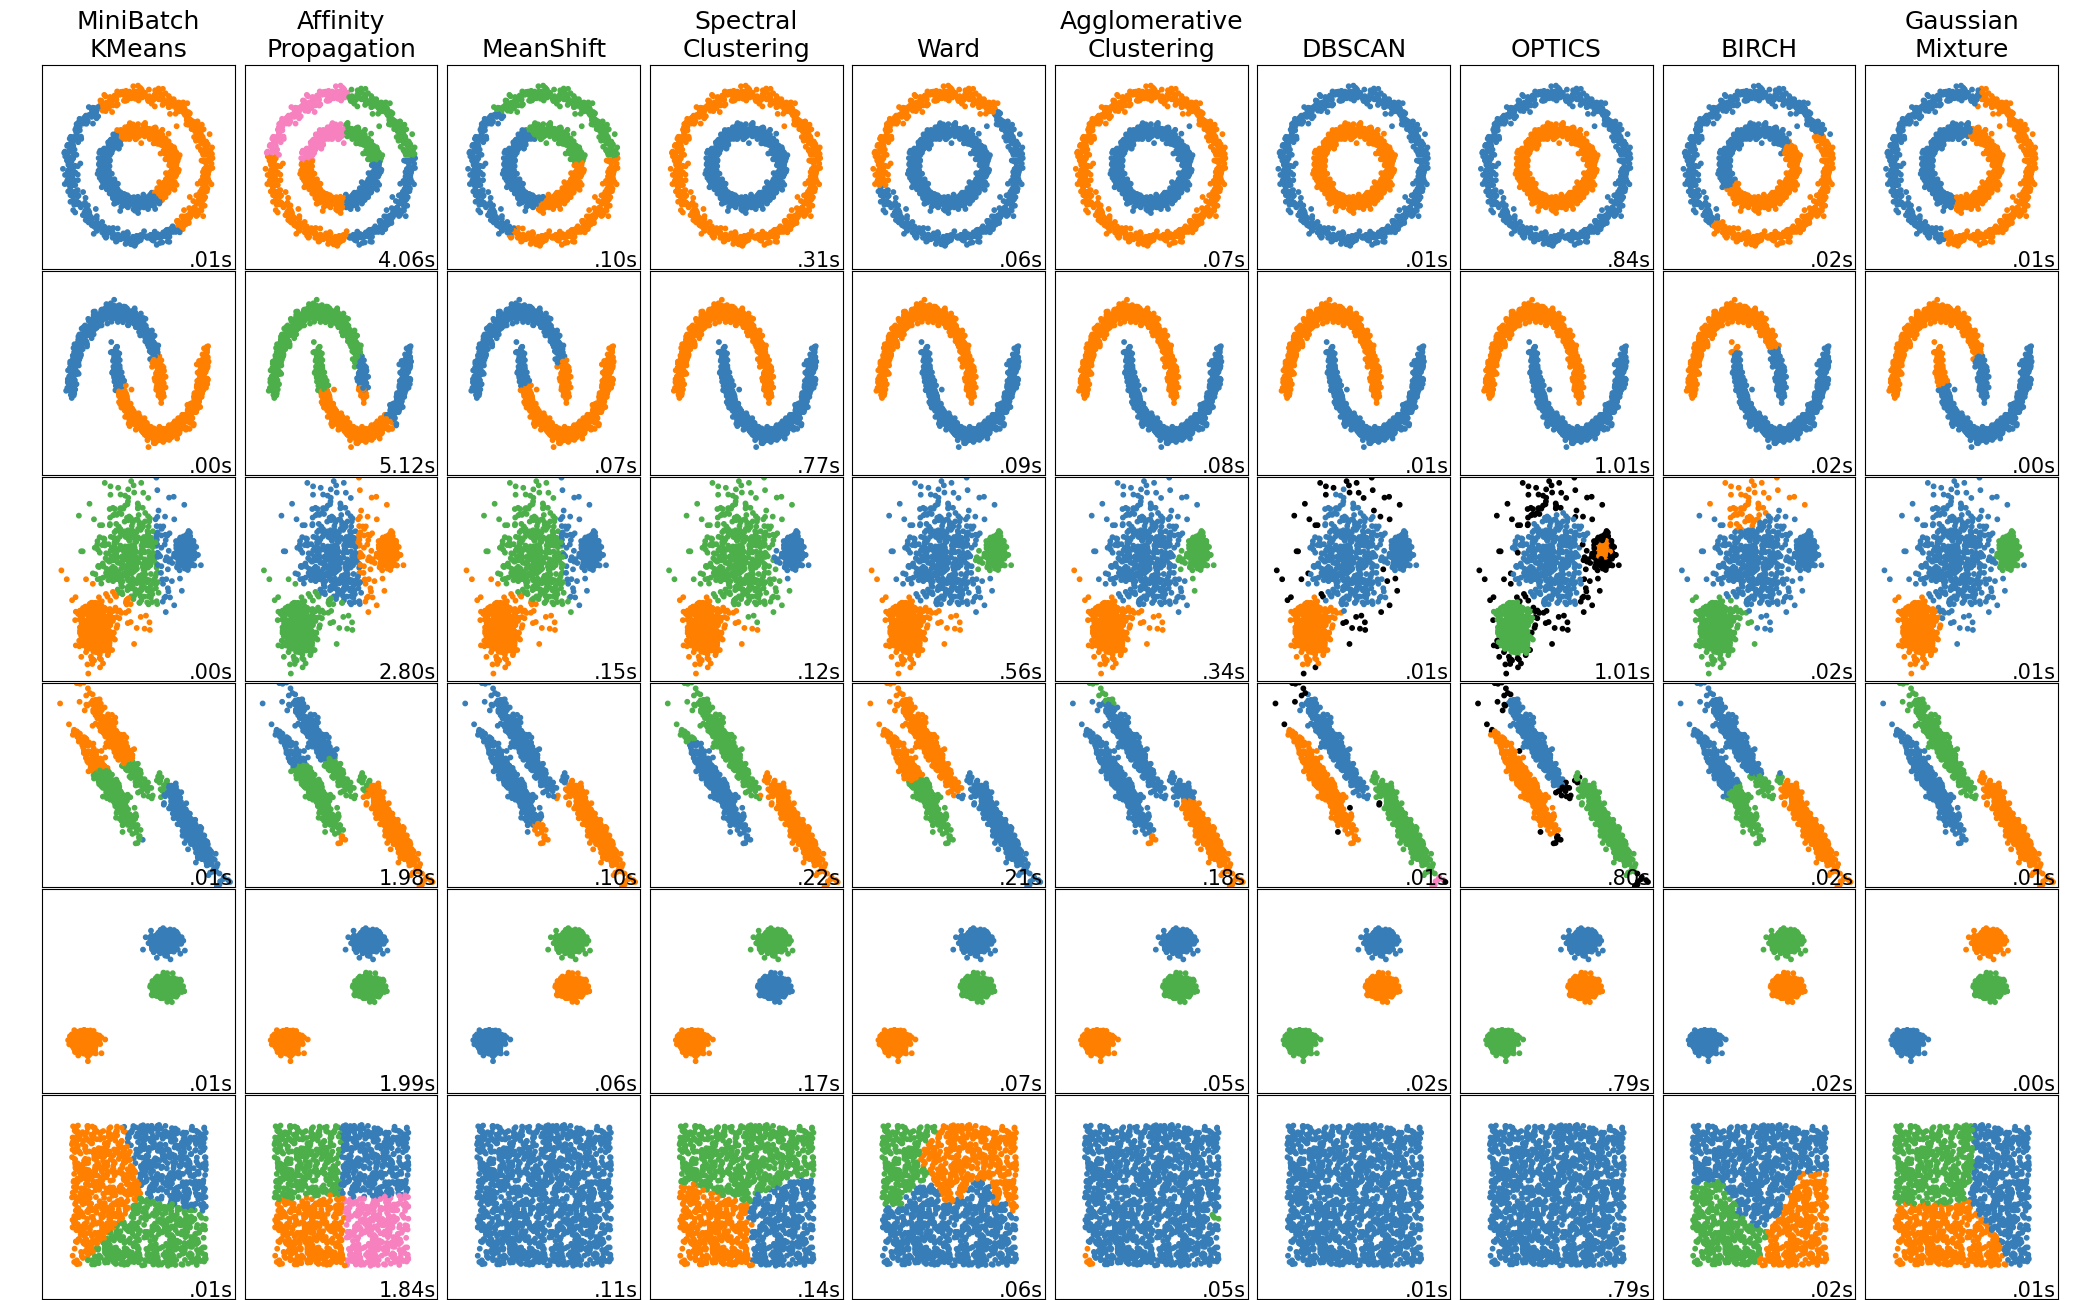
\includegraphics[width=\textwidth]{clusters.png}
        \caption[]{Clusterisation algorithms used on sample two-dimensional data sets to demonstrate resultant clusters.}
        \label{fig:ClusterResults}
    \end{center}
\end{figure}

As Figure~\ref{fig:ClusterResults} demonstrates, there are multiple different interpretations of the solution to the problem of clustering. The makers of the Scikit learn package also discuss the scalability of each algorithm \cite{SciClus}. In order to prepare a high number of features (beyond the two used within this section for demonstration) and large number of data points, it is required that the algorithm scales accordingly. Further, for an adaptive process, it is more suitable for an algorithm to be adaptive to differing distribution. This limits the suitable algorithms to K-Means, Ward and Birch - columns one, five, and nine of Figure~\ref{fig:ClusterResults} respectively. Results for Birch can be seen in Figure~\ref{fig:clusterPhantom}. This appears do well, although it must be noted that this is likely due to the similarity between Monte Carlo (random) sampling, and clusterisation. I.e. areas distant from previously gathered points face a high chance of sampling.

\begin{figure}[H]
    \begin{center}
        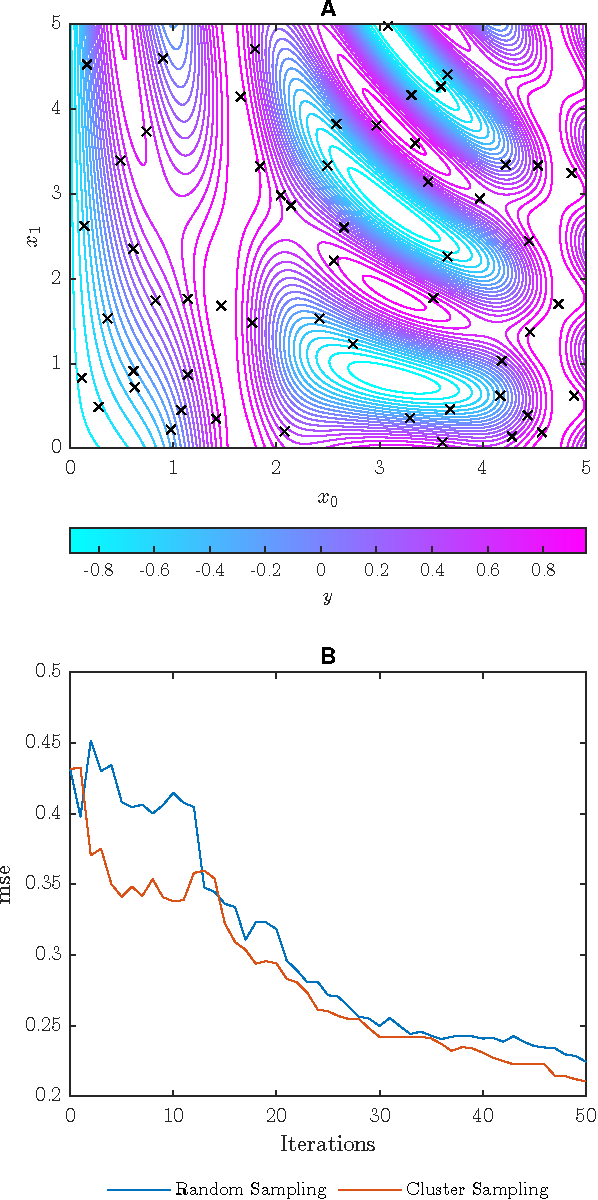
\includegraphics{clusterPhantom.pdf}
        \caption[Cluster Hotspot Sampling Illustration]{The outcome of the investigating the areas of using a cluster hotspot sampling methodology. An initial set of 5 random points was provided, and 50 further iterations were then carried out of sample size 1. A) Demonstrates the final set of points tested by the algorithm and B) shows the change in the mean squared error for the algorithm after each iteration.}
        \label{fig:clusterPhantom}
    \end{center}
\end{figure}

\subsection{Estimated Future}
These methods attempt to minimise a future attribute of the model. This works by predicting changes given with the inclusion of more data with a higher degree f theoretical underpinning that the sampling methods discussed thus far.

\subsubsection{Expected Model Change}
As the name implies, this method chooses points which are likely to have the largest impact on the final model. By instigating each potential point, the impact on the eventual model can be found. However, this requires a method for quantifying the model change.

\textcite{Set08,Set09} investigate models which can be trained "online": i.e. models which can use the previous iteration to reduce the time taken for convergence. They present a method called "Expected Gradient Length" (EGL) which has a couple of prerequisites: \textbf{1)} A probabilistic model is used \textbf{2)} Linear gradient based optimisation is used \textbf{3)} The model can be improved from previous iterations. Given these prerequisites, the problem becomes less computationally inexpensive given a small dataset or extensive parallelisation, and scales as $\mathcal{O}(n)$. However, it does have the distinct drawback of requiring close control of the data models used. Here, the length of the training gradient (the gradient used in re-fitting the parameters with gradient based optimisation) can be used as a measure of model change. In the case of a small model change, as is expected, the length of the training gradient can be written as ${\left\|\nabla{}l(\langle{}x, y_i\rangle{};\theta{})\right\|}$. Combining this with the probability distribution of $y$, the next sample to undergo labelling is given by (\ref{eq:EGL}).

\begin{equation}
    \label{eq:EGL}
    x_{EGL}^*=\argmax_x{\sum_i{P(y_i|x;\theta{})\left\|\nabla{}l(\langle{}x, y_i\rangle{};\theta{})\right\|}}
\end{equation}


\section{Batch Active Learning}
Little literature exists with respect to batch active learning. Naive implementation exist whereby the methods explored earlier present a stack of data points to be chosen, and the top $N$ are used. However, this method does not take into account the equivalence of the data points. This can be seen by the formation of clusters within the broad and uncertainty sampling methods, although it is not present within the clusterisation algorithm.

\begin{figure}[H]
    \begin{center}
        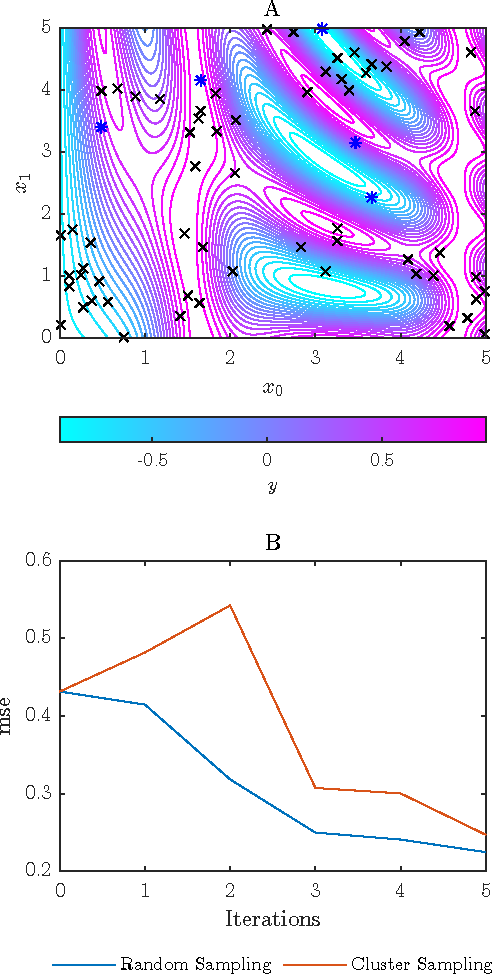
\includegraphics{broadrodPhantom.pdf}
        \caption[Batch Uncertainty Sampling]{The outcome of the investigating the areas of using uncertainty sampling. An initial set of 5 random points was provided, and 5 further iterations were then carried out of sample size 10. A) Demonstrates the final set of points tested by the algorithm and B) shows the change in the mean squared error for the algorithm after each iteration.}
    \end{center}
\end{figure}

% \begin{figure}[H]
%   \begin{center}
%     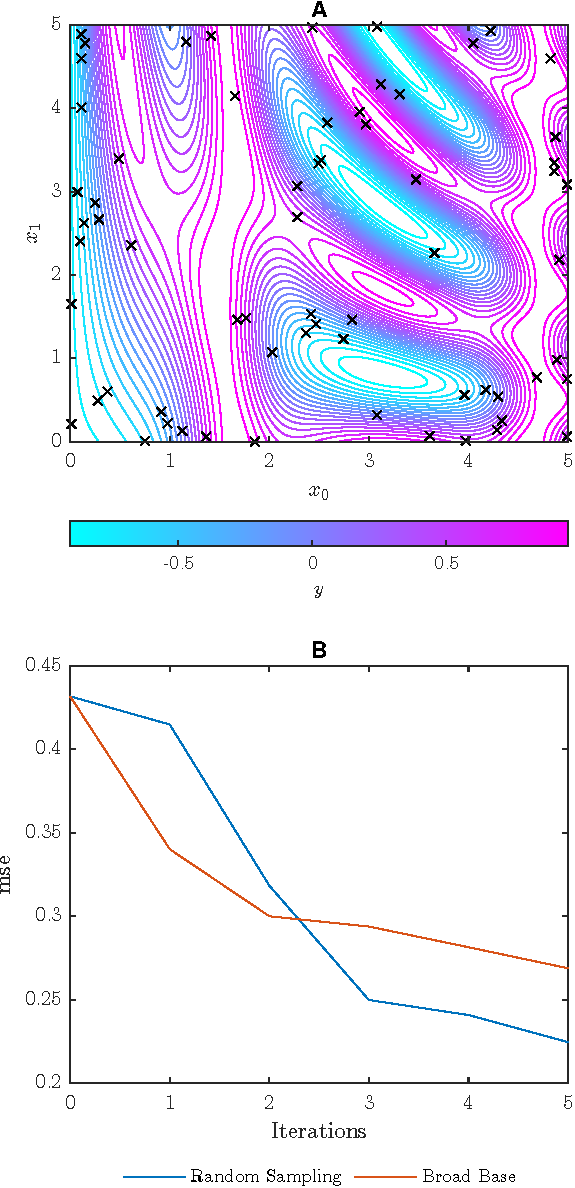
\includegraphics{batchbroadPhantom.pdf}
%     \caption[Batch Broad-Base Sampling]{The outcome of the investigating the areas of using broad-base sampling. An initial set of 5 random points was provided, and 5 further iterations were then carried out of sample size 10. A) Demonstrates the final set of points tested by the algorithm and B) shows the change in the mean squared error for the algorithm after each iteration.}
%   \end{center}
% \end{figure}

\begin{figure}[H]
    \begin{center}
        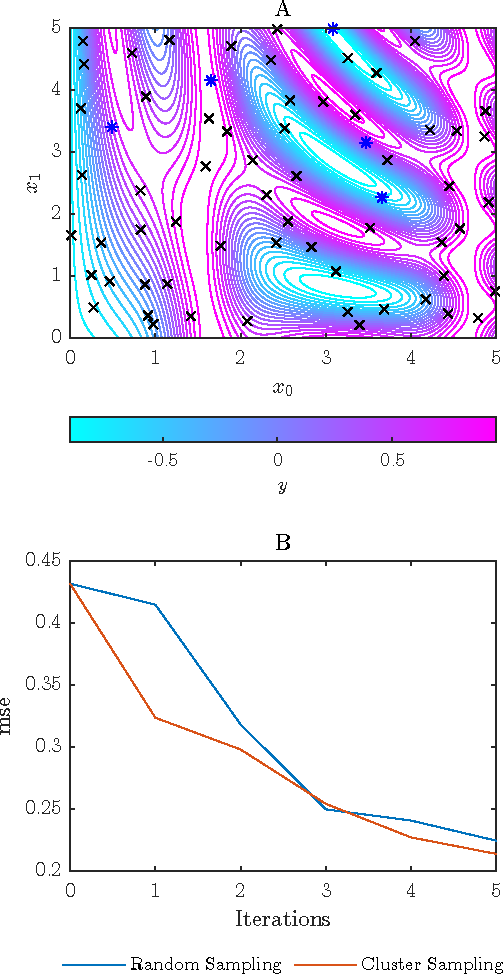
\includegraphics{broadClusterPhantom.pdf}
        \caption[Batch Cluster Sampling]{The outcome of the investigating the areas of using cluster sampling. An initial set of 5 random points was provided, and 5 further iterations were then carried out of sample size 10. A) Demonstrates the final set of points tested by the algorithm and B) shows the change in the mean squared error for the algorithm after each iteration.}
    \end{center}
\end{figure}


It stands to reason that the area which has the highest uncertainty will see this for the data points nearest neighbours. Thus, this singular data point suffers the potential of being surrounded by $N-1$ other data points. The benefit this provides in fitting the model is thus extremely limited, and only slightly greater than if one data point had been chosen. A simple fix would be to simulate the model after 1 iteration, and select the next point from here. By doing this $N-1$ times, a better solution may be found, although this may prove to be computationally expensive.

\subsection{BatchBALD}
\textcite{BatchBALD} propose an algorithm named BatchBALD (Batch Bayesian Active Learning by Disagreement). Demonstrating for sample size of 10 an improvement compared to random sampling in optical character recognition. In doing so, they use complex Bayesian Neural Networks and apply the problem to categorical data.

\section{Drug Data for Machine Learning}
There are numerous data categories that can be used to represent a chemical in a suitable form for machine learning. Indeed, the field of chemoinformatics is dedicated to the pursuit of describing chemicals for computational models. Each of these methods have various strengths and weaknesses. Some are directly based upon the chemical structure whereas others are based upon physical properties. These can be combined to produce models with high predictive capabilities.

\subsection{Physical Properties}
A selection of physical properties from chemicals are known, from melting points to solubility. Many of these provide important aspects for consideration and allow human scientists to predict interactions, especially when determining new drugs. These data are often reported in tables within textbooks such as Perry's Chemical Engineering Handbook or provided through software \cite{CHEMBL,Perrys}.

Several of these data can be predicted through theoretical models, although the difficulty increases for larger molecules. For example, models exist for density predictions, but predicting the $\mathrm{LD_{50}}$ of a drug is  far more challenging task. Indeed, even with animal testing, this property is deemed difficult to truly assess.

Within drug discovery, physical and biological properties are usually the sought after labels. An example of this is supplied by \textcite{CHEMBL} with a custom property named pChEMBL, as defined by (\ref{eq:pChEMBL}) where "|" is synonymous with "or". Values are expected to be between 2 and 12, although these are not limited. Indeed, values even be negative, although this is rare and unlikely.

\begin{equation}
    \label{eq:pChEMBL}
    \mathrm{pChEMBL}=-\log_{10}{\left(\mathrm{IC_{50}}|\mathrm{XC_{50}}|\mathrm{EC_{50}}|\mathrm{AC_{50}}|\mathrm{Ki}|\mathrm{LD_{50}}|\mathrm{Potency}\right)}
\end{equation}

\subsection{Fingerprints}
Another methodology is to develop a fingerprint: a unique code based on the chemical structure, either of the atomic arrangement, or by the electron cloud distribution. The latter of these is more fundamental to the activity of molecules but far harder to calculate. Indeed, for accurate representation of the latter, both atomic structure is needed \textit{and} solutions for the Schrödinger equations corresponding to molecule in question.

According to \textcite{Cap20}, the most popular fingerprint in use are Morgan Fingerprints, a form of Extended Chemical Fingerprint (ECFP). ECFPs use a simple algorithm in order to generate a unique identifier, as described by \textcite{Mor2020}:

\begin{enumerate}
    \item \textbf{Initial Assignment}: Each atom has an integer assigned as an identifier.
    \item \textbf{Iterative Updating}: Updating the identifier assigned to atoms based on adjacent atoms and structural duplications.
    \item \textbf{Duplicate Removal}: Duplicate features are removed for hashing.
\end{enumerate}

The iteration process involves each atom and adjacent atoms sharing numbers before in an array. A hash function is applied to this array and becomes the atoms new identifier. Fingerprints of this class are labelled according to the number of iterations, $n$, with the final name given as ECFP\_$\langle{}2n\rangle{}$. Morgan fingerprints, the most common form, are thus also called ECFP\_4 \cite{Cap20, Mor2020}. Thus, these come under the remit of fingerprints based upon two-dimensional chemical structure, rather than three-dimensional or even electron distribution. Morgan fingerprints are readily available for millions of compounds from the publicly accessible ChEMBL database \cite{CHEMBL}.

% Alternative common fingerprints include SMILES, InChI, and the MDL molfile.
%!TEX root = ../thesis.tex
%*******************************************************************************
%****************************** Third Chapter **********************************
%*******************************************************************************
\chapter{Methodology}
% **************************** Nomenclature **********************************
\nomenclature[d-1-XTrain]{$X_\mathrm{train}$}{Datasets used for training the algorithms}
\nomenclature[d-1-XTest]{$X_\mathrm{test}$}{Datasets used to provide a score for the algorithms}
\nomenclature[d-2-xunknown]{$x_\mathrm{unknown}$}{Data points where the true label is not available to the algorithms used}
\nomenclature[d-2-xknown]{$x_\mathrm{known}$}{Data points where the true label is available to the algorithms used}
\nomenclature[d-3-yunknown]{$y_\mathrm{known}$}{True labels available to the algorithms used}
\nomenclature[d-3-yunknown]{$y_\mathrm{unknown}$}{True labels unavailable to the algorithms used}
\nomenclature[d-3-yunknown]{$n$}{The number of samples per iteration}
% \nomenclature[u-3-ypredict]{$y_\mathrm{predict}$}{Predicted labels by the algorithm}
% **************************** Define Graphics Path **************************

\graphicspath{{Chapter3/Figs/Vector/}{Chapter3/Figs/}}
\section{Outline}
\subsection{Data}
Each dataset used consists of a 1024 bit Morgan fingerprint for the features and these associated pChEMBL values. The sets used for parameter fitting and score reporting make up a set of 2094 files from \textcite{CHEMBL}. These were filtered to prevent datasets with fewer than 1000 entries to be admitted into the main script.

Morgan fingerprints were chosen due to the ease in which it is to calculate the vectors, the popularity of them within the chemoinformatics sphere, and the success enjoyed by others when using them for predictive purposes. It was decided that physical properties would not be used as this could increase the onus on data sanitation and preparation rather than active learning.

\subsection{Custom Algorithms}
As well as the algorithms used mentioned in Chapter~\ref{ch:2}, several custom algorithms were developed and added to the testing set. These methods do use parameters, and so require the minimisation technique. Addtionally, these algorithms take a composite methodology, using other active learning methods in order to reach a conclusion, so some concepts will be assumed knowledge for Chapter~\ref{ch:2}.

\section{Computational Methodology}
The methodology presents a novel means of assessing different parametrised active learning methods on existing data sets, allowing for a robust answer into the use of active learning in drug rediscovery. Results can thus be given with a given belief. This approach has taken principles commonly used in machine learning and applied it to more traditional algorithmic methods.
\\
Firstly, a collection of pre-existing data sets, $X$, are used. $X$ is then split into two sub sets: $X_{\mathrm{train}}$ and $X_\mathrm{test}$. Similarly to machine learning, the former of these subsets is used in fitting the parameters of the equation, and the latter is used to provide a result without the risk of data leakage into the training set. This is represented in []. Parallelisation is used to efficiently train the algorithms allowing the time for training to be $\sim{}\mathcal{O}(c)$.
\\
Examining the smaller details, each algorithm is provided with the sets $x_\mathrm{known}$, $y_\mathrm{known}$, and $x_\mathrm{unknown}$. Various algorithms are given these sets and allowed to generate a subset of $x_\mathrm{unknown}$ to be added into $x_\mathrm{known}$ alongside corresponding $y_\mathrm{known}$. This can then repeat until a predefined stopping point is reached. Scores are reported using a weighted mean squared error [] based upon $y_\mathrm{predict}$ for all $x$. This is similar to a standard machine learning methodology with a couple of differences. Firstly, no distinction is made between the training and testing set within a dataset contrary to standard practice. This is due to two reasons. Firstly, the datasets are not large enough for an accurate representation of the data within the testing set, and secondly, the scoring to each dataset is not used within the machine learning algorithms to fit parameters as is usually the case. All algorithms used rely upon a simple custom composite model to allow for flexibility and consistency.
\\
In Section [], it was discussed that there are various methodologies of representing chemicals and drugs. ... (if time)

\subsection{Integral Functions and Classes}
Several key methods and classes are required for the smooth operation of the computational frameworks used

\subsection{Custom Base Functions}
\subsubsection{\lstinline{Split}}
The\lstinline{split} function allows for each dataset to be split into $x_\mathrm{known}$, $y_\mathrm{known}$, $x_\mathrm{unknown}$, and $y_\mathrm{unknown}$, as demonstrated in Figure \ref{fig:Split}. This is required as a fundamental step for the algorithmic testing. To demonstrate the validity of this function, ...

    \begin{figure}
        \begin{center}
            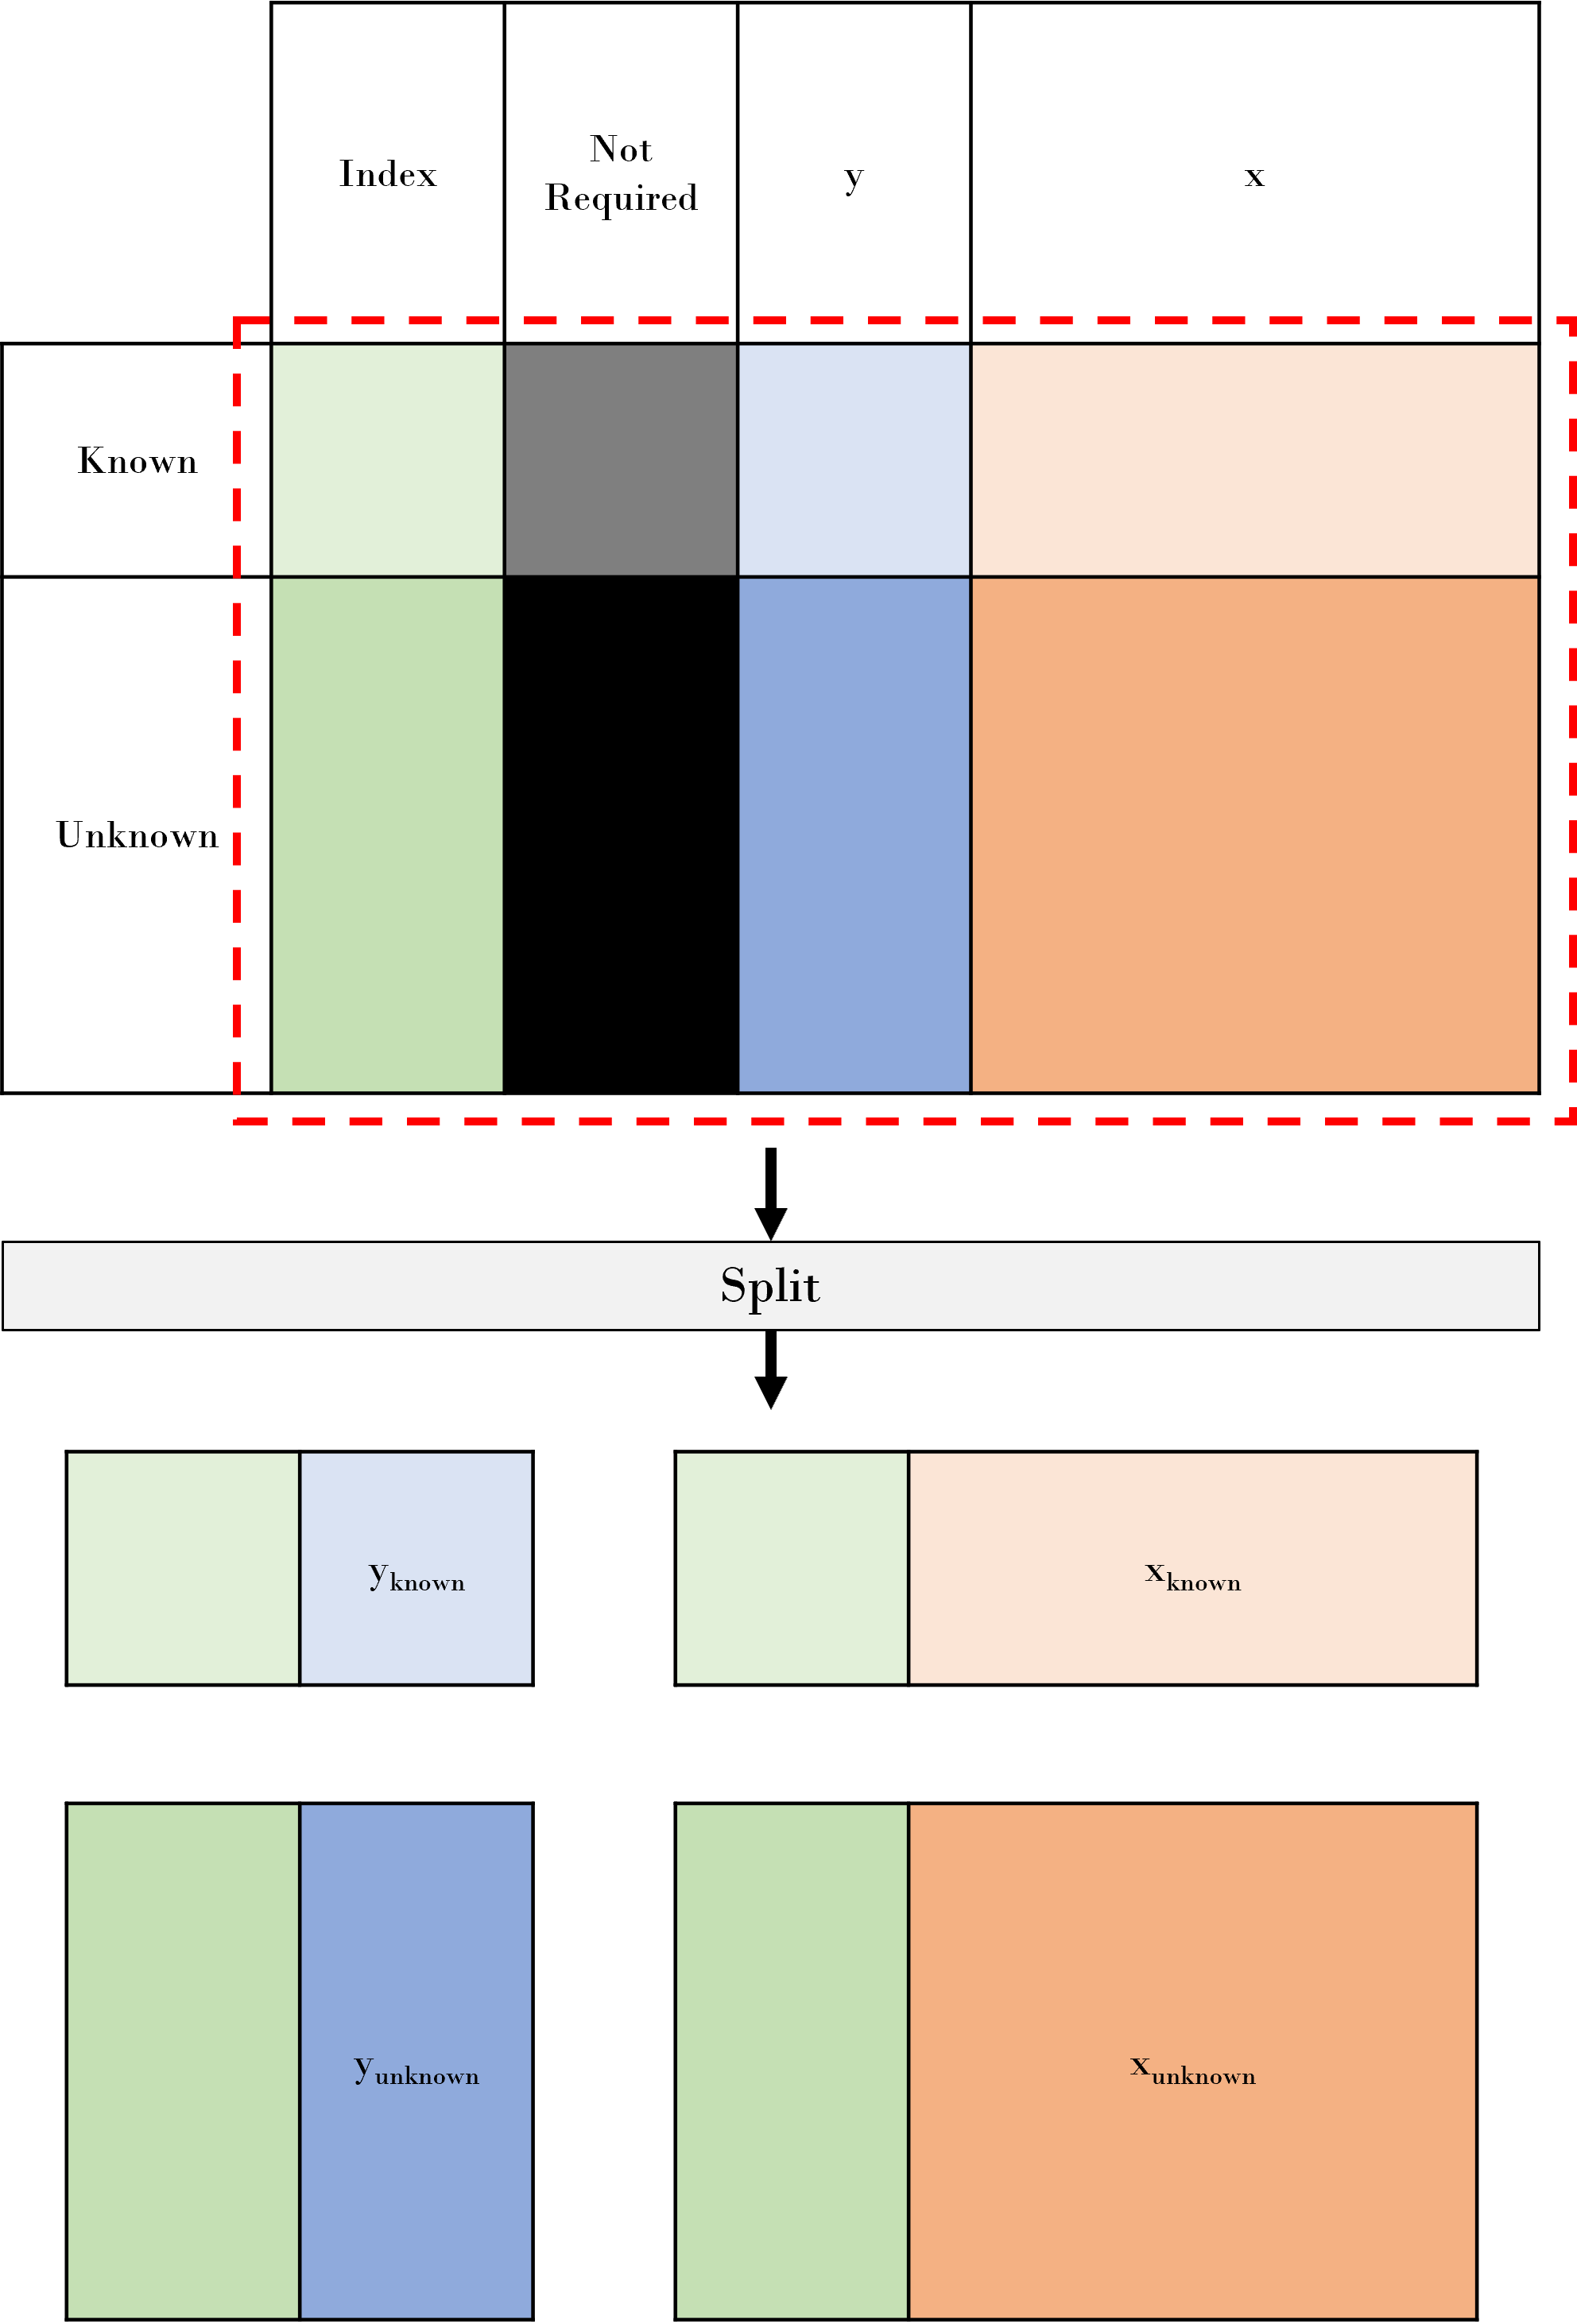
\includegraphics[width=\textwidth]{split.png}
        \end{center}
        \caption[Representation of the split function]{Graphical representation of the\lstinline{split}function. The red dashed boundary represents the input (additional colour coding has been performed to assist the reader in understanding the transposition of the base components).}
        \label{fig:Split}
    \end{figure}


    \subsubsection{\lstinline{Repartition}}
    Upon each iteration, the sets provided to the algorithms need to be repartitioned to allow for the continual operation of the algorithm. This consists of two parts: expanding the known sets and removing entries from the unknown sets.

    \subsubsection{\lstinline{Model}}
    The machine learning model is the only custom class used. Here, a similar structure is used when compared with sci-kit's machine learning \cite{scikit}, as is demonstrated in Table~\ref{tab:Model}. To manage this, it has four methods:\lstinline{__init__},\lstinline{fit},\lstinline{predict}, and\lstinline{predict_error}. The last of these is not seen in all sci-kit's machine learning models and is reserved for those which can report a certainty of prediction. Here, this was achieved by taking a standard deviation of the models.

    \begin{table}[h]
        \centering
        \begin{tabular}{@{}ccc@{}}
            \toprule
                                                   & Name                         & Description                                                                                      \\ \midrule
            Attributes                             & Models: List                 & List of models to be used in composite                                                           \\ \midrule
            \multirow{3}{*}{Methods}               & fit(X: int[][], Y: double[]) & Fits the models in Models                                                                        \\
                                                   &
            predict(X: int[][]): double[]          &
            \begin{tabular}[c]{@{}c@{}}Takes a set of labels and returns mean\\ predicted label from all the models.\end{tabular}                                                    \\
                                                   &
            predict\_error(X: int[][]): double[][] &
            \begin{tabular}[c]{@{}c@{}}Takes a set of labels and returns the mean\\ predicted label from all the models and\\ standard deviations of model predictions.\end{tabular} \\
            \bottomrule
        \end{tabular}
        \caption{Schema for the Model Class.}
        \label{tab:Model}
    \end{table}

    The models used for the composite model were \dots which will be consistent across all algorithms. This allows direct comparison of the algorithms without interference from machine learning models used.

    \subsubsection{\lstinline{Validate}}
    This is a simple method with greater potential than has been explored. By providing this as a separate method, a more computationally intensive validation model could be used without interference as parallelisation could be exploited. However, as it currently stands, it returns the weighted mean squared error using the standard method provided by [].

    \subsection{Active Learning Algorithms}

    \subsubsection{Dumb}

    The dumb algorithm, also referred to as random sampling or Monte Carlo sampling, refers to an algorithm that calls upon random samples to be tested. This represents the computationally least expensive approach, and is thus used as a baseline in comparing other algorithms. Since the datasets are shuffled prior to being used, the algorithm is extremely simple, as demonstrated in Algorithm~\ref{alg:MC}.

    \begin{algorithm}[h]
        \KwData{$X_\mathrm{unknown}$}
        \KwResult{$X$ ordered according to priority for sampling}
        \Return{$\mathrm{ones\_like}(X_\mathrm{unknown})$}
        \caption{Uncertainty Sampling Selection}
        \label{alg:MC}\SetAlgoLined
    \end{algorithm}

    \subsubsection{Greedy}
    Since the largest activity is sought, a methodology proposed is to simply seek the predicted highest label. Here, the predict() method (see Table~\ref{tab:Model}) was used to return a prediction and a standard deviation. The indices of $x_\mathrm{unknown}$ were then returned, ordered descending with respect to the afore mentioned standard deviations.

    \begin{algorithm}[h]
        \KwData{$X_\mathrm{known}$, $Y_\mathrm{known}$, $X_\mathrm{unknown}$, Model}
        \KwResult{$X$ ordered according to priority for sampling}
        Model.fit($X_\mathrm{known}$, $Y_\mathrm{known}$)\;
        prediction = Model.predict\_error($X_\mathrm{unknown}$)\;
        \Return{$-\mathrm{prediction}$}
        \caption{Greedy Sampling Selection}
        \label{alg:greedy}\SetAlgoLined
    \end{algorithm}

    \subsubsection{Region of Disagreement}
    Similarly to the region of disagreement method, this is a very simple algorithm. Here, the predict\_error() method (see Table~\ref{tab:Model}) is used to return a prediction and a standard deviation. The prediction is ignored, and instead the standard deviation is returned, multiplied by $-1$ to ensure the largest uncertainty has the lowest "score". This is shown in \ref{alg:rod}.

    \begin{algorithm}[h]
        \KwData{$X_\mathrm{known}$, $Y_\mathrm{known}$, $X_\mathrm{unknown}$, Model}
        \KwResult{$X$ ordered according to priority for sampling}
        Model.fit($X_\mathrm{known}$, $Y_\mathrm{known}$)\;
        \_, error = Model.predict\_error($X_\mathrm{unknown}$)\;
        \Return{$-\mathrm{error}$}
        \caption{Uncertainty Sampling Selection}
        \label{alg:rod}\SetAlgoLined
    \end{algorithm}

    \subsubsection{Hotspot Cluster I}
    This is the first of the clustering algorithms and the first parametric algorithm. This algorithm is based upon the ideology presented in Section~\ref{sec:litRevDH}, and is shown in Algorithm~\ref{alg:cluster1}. Here, $c$ is the number of cluster sought, and is a parameter that requires fitting. Bounds can be placed upon this. The lower limit can be set as the number of known data points, and the upper as the total number of data points in the data set, although it is hypothesised that beyond the sum of the known points and the samples sought would make little, to no difference. To test this hypothesis, the upper limit will be set at $\mathrm{len}(X_\mathrm{unknown})+1.5n$. The combined limits have been shown in \ref{eq:limsClust1}.

\begin{equation}
    \label{eq:limsClust1}
    {\mathrm{len}(X_\mathrm{known})<c<\mathrm{len}(X_\mathrm{unknown})+1.5n}
\end{equation}

\begin{algorithm}[h]
    \KwData{$X_\mathrm{known}$, $X_\mathrm{unknown}$, $c$}
    \KwResult{$X$ ordered according to priority for sampling}
    combined\_x = concat(X, x)\;
    clusters = cluster(number\_of\_clusters=$c$)\;
    clusters.fit(combined\_x)\;
    predicted\_custers = clusters.predict($X_\mathrm{unknown}$)\;
    distances = clusters.distance\_to\_nearest\_centroid($X_\mathrm{unknown}$)\;

    \Return{$-\mathrm{error}$}
    \caption{Uncertainty Sampling Selection}
    \label{alg:cluster1}\SetAlgoLined
\end{algorithm}

\subsubsection{Hotspot Cluster II}
This is similar to the previous algorithm with one difference, the labels. Both known and predicted are used within the algorithm to ...

\subsubsection{Hotspot Cluster III}
The final hotpsot clustering algorithm also encompasses the uncertainty from the prediction models.

\subsection{Training Framework}
\blindtext[1]
\subsubsection{Parallelisation}
\blindtext[1]
\subsubsection{Minimisation}
\blindtext[1]
%!TEX root = ../thesis.tex
%*******************************************************************************
%****************************** Fourth Chapter **********************************
%*******************************************************************************
\chapter{Results}

% **************************** Define Graphics Path **************************

\graphicspath{{Chapter4/Figs/Vector/}{Chapter4/Figs/}}

\section{Non-Parametric}
Non-parametric equations have the benefit of not requiring the minimisation function. Due to this, all testing of these algorithms were undertaken on a standard laptop. These also tend to be the easiest to implement, as uncovered in Chapter~\ref{ch:method}. Particularly important is the Monte Carlo method as this allows shows what should be a minimum baseline to achieve.

\subsection{Monte Carlo}
The first non-parametised algorithm discussed in Chapter~\ref{ch:method} was the Monte Carlo method. Due to the non-parametric nature of this algorithm, execution was simply carried out on the test data set. Results are presented in Figure~\ref{fig:MCTestSet}, demonstrating a final weighted mse of $0.92\pm{}0.43$.
\begin{figure}[h]
    \begin{center}
        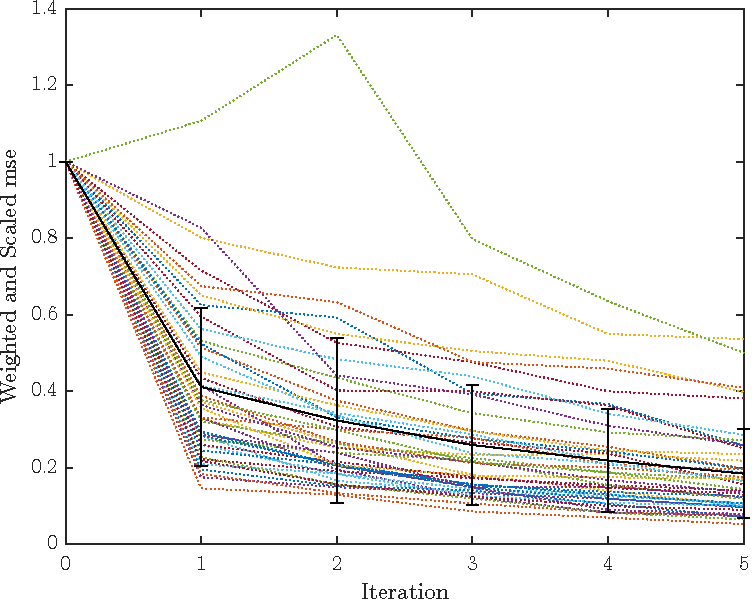
\includegraphics{dumb1.pdf}
        \caption[Monte Carlo]{Results of Monte Carlo sampling on the test datasets. Dotted lines represent the individual scoring for the data sets and the solid line shows the mean results at each iteration with error bars of 1 standard deviation.}
        \label{fig:MCTestSet}
    \end{center}
\end{figure}

\subsection{Greedy}
Likewise, the greedy algorithm was tested, with results presented in Figure~\ref{fig:GreedyTestSet}. Here, a final weighted mse of $0.95\pm{}0.37$ was found indicating a worse scoring despite more precise results when compared to Monte Carlo - the base case.
\begin{figure}[h]
    \begin{center}
        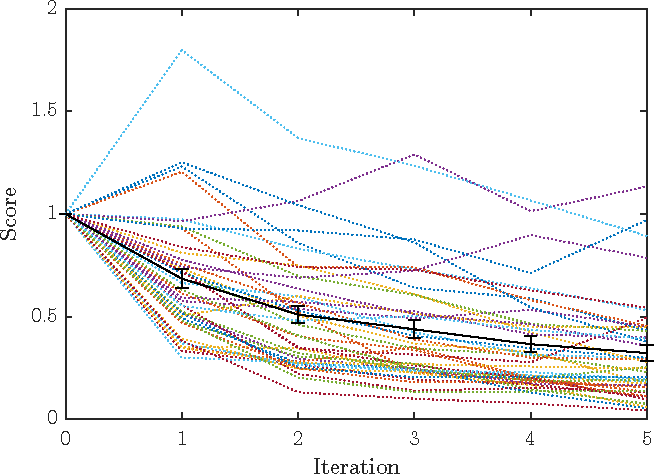
\includegraphics{greedy1.pdf}
        \caption[Greedy]{Results of greedy sampling on the test datasets. Dotted lines represent the individual scoring for the data sets and the solid line shows the mean results at each iteration with error bars of 1 standard deviation.}
        \label{fig:GreedyTestSet}
    \end{center}
\end{figure}

\subsection{ROD Sampling}
The final non-parametic algorithm to be tested was ROD. A final weighted mse of $0.67\pm{}0.23$, over performing the previous two algorithms in both accuracy and precision.

\begin{figure}[h]
    \begin{center}
        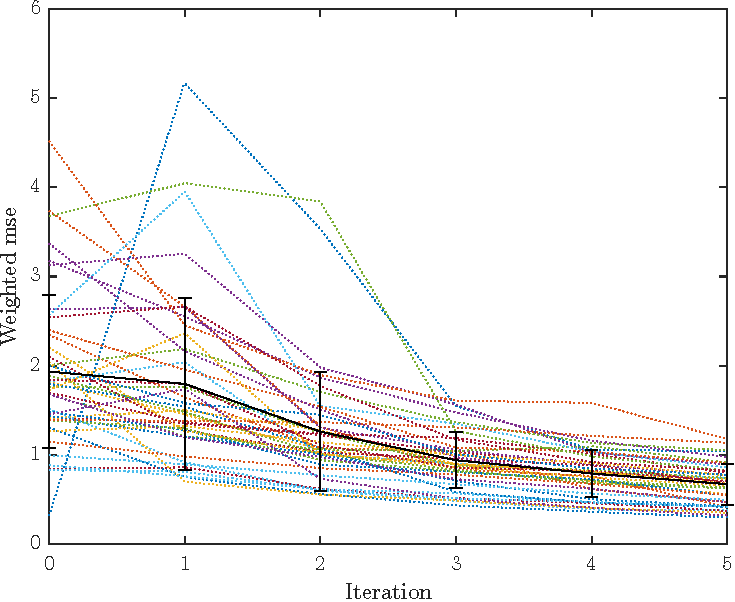
\includegraphics{rod1.pdf}
        \caption[ROD]{Results of ROD sampling on the test datasets. Dotted lines represent the individual scoring for the data sets and the solid line shows the mean results at each iteration with error bars of 1 standard deviation.}
        \label{fig:RODTestSet}
    \end{center}
\end{figure}

\section{Parametric}
Parametric algorithms require a minimisation procedure on the training set. This leads to a computationally challenging script, and for this the author is grateful for the services provided by the HPC \cite{HPC}.
\subsection{Hotspot Clusters}
\blindtext[1]
\subsection{ROD with Greed}
When testing the ROD with greed sampling method, it was found that despite the weighting towards higher value targets, no improvement was seen over ROD with an $\alpha{}=0$ according to \ref{eq:rodAndGreed}.

\begin{figure}
    \begin{center}
        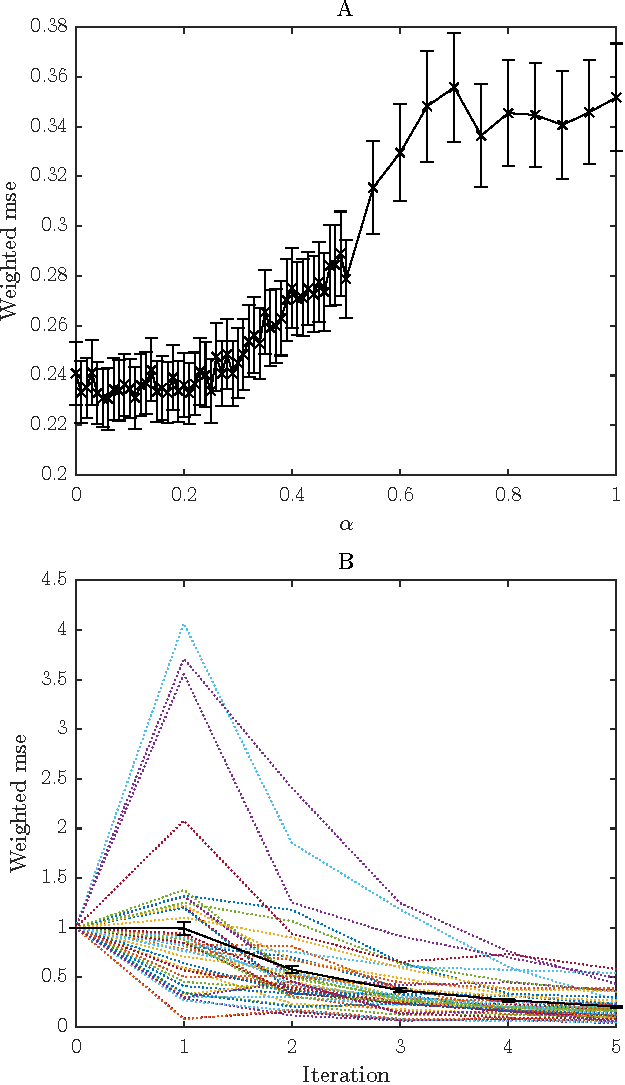
\includegraphics{rodGreedParam.pdf}
    \end{center}
\end{figure}

\section{Special Case: COVID-19}
%!TEX root = ../thesis.tex
%*******************************************************************************
%****************************** Third Chapter **********************************
%*******************************************************************************
\chapter{Discussion}

% **************************** Define Graphics Path **************************

\graphicspath{{Chapter5/Figs/Vector/}{Chapter5/Figs/}}


\section{Non-Parametric}
Three algorithms tested of non-parametric variety producing several noticeable results. Firstly, Monte Carlo sampling outperformed both Greedy and RoD sampling. This is demonstrated convincingly through Figure~\ref{fig:nPComp} where results from the greedy results suggest the worst accuracy.

Despite the greedy algorithm demonstrating the worst accuracy, interesting results were shown with RoD sampling. Poor selection is evidently present with the first sample set, although rapid improvement quickly follows. Indeed, after the first iteration, the learning rate is superior to the other two algorithms. An extra iteration may indeed have seen RoD surpassing Monte Carlo. This is expected as the ROD algorithm specifically targets regions of the model which are challenging causing the largest changes towards proper fitting.

Both RoD and greedy sampling are suspected to suffer from clusterisation whereby data points similar to each other in the feature space are sampled within the same batch, thus reducing the total information conveyed per batch operation. This is believed to be particularly costly with the first iteration as the model will heavily overfit to the new cluster it has sampled. The random nature of Monte Carlo reduces this prospect, hence the apparent promising performance of a random sampling methodology. Evidence to this is shown in Figure~\ref{fig:MCTestSet}, Figure~\ref{fig:GreedyTestSet}, and Figure~\ref{fig:RODTestSet}.

\begin{figure}[h]
    \begin{center}
        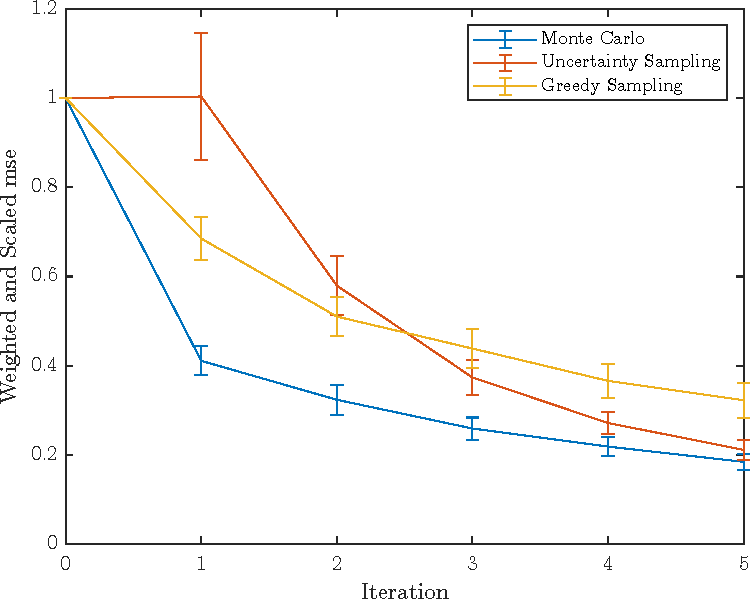
\includegraphics{nonParamComp1.pdf}
        \caption[Non-parametric comparison]{Comparison of different non-parametric algorithms with standard deviations represented as error bars.}
        \label{fig:nPComp}
    \end{center}
\end{figure}

This demonstrates a danger with Batch Active Learning. It is very easy to produce a learning algorithm which actually performs worse than random screening.

\section{Parametric}
Different classes of parametric algorithms were tested. The first of these is a first order composite algorithm, RoD with Greed: i.e. uses different active learning algorithms as a base. The second is a clustering algorithm with the number of clusters left as a parameter. The third is a second order composite active learning algorithm which combines the other two parametric functions, affectionately named the Holy Trinity. A constant improvement is seen throughout these algorithms, with the Holy Trinity performing the best.

\begin{figure}[h]
    \begin{center}
        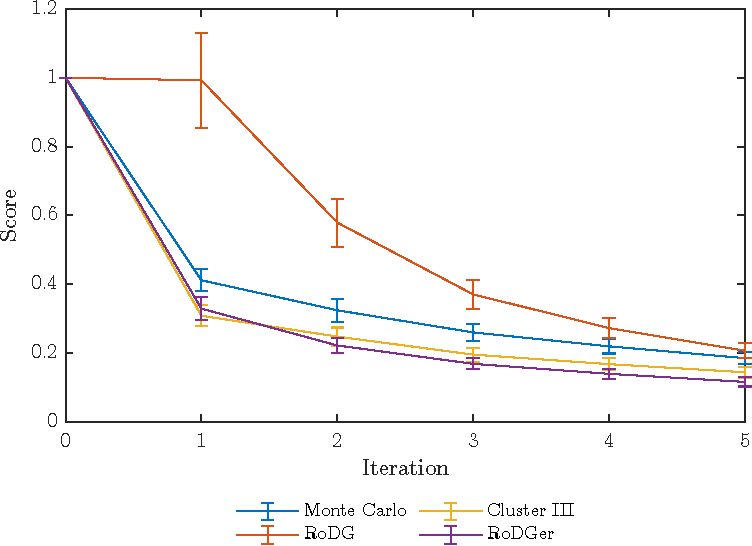
\includegraphics{paramComp1.pdf}
        \caption[Non-parametric comparison]{Comparison of different parametric algorithms with standard deviations represented as error bars.}
        \label{fig:pComp}
    \end{center}
\end{figure}

Several points of interest are highlighted with these results. Firstly, despite improving upon RoD, RoD with Greed is still beaten by Monte Carlo sampling. Again, the methodology suffers from clustering of points. This is shown with the ability of Cluster III outperforming Monte Carlo. The progression through the different cluster algorithms also sees improvement with progression, as anticipated.

The sampling process of the Cluster III algorithm demonstrates its ability at outperforming the random sampling methodology of Monte Carlo even within the first iteration. The Holy Trinity algorithm sacrifices some of this initial performance for longer term gain, as shown by the worse performance after the first iteration. By the second iteration, the difference becomes insignificant, with the error for each algorithm. By the end of the fifth iteration, the Holy Trinity algorithm convincingly outperforms the other algorithms.

Upon investigation of the parameters settled upon within these several points arise. Firstly with RoD with Greed, at low $\alpha$, the score appears uncorrelated with $\alpha$, only experiencing a significant rise with $\alpha{}>0.4$. Thus, it can be surmised that RoD is the driving force, with evidence given by the final scores for RoD and RoD with Greed algorithms arising within error of each other.

On the other hand, the sensitivity of Cluster III is extremely low to cluster size, demonstrated by Figure~\ref{fig:clusterTest}. Here, no significant change is observed within the significant parameter range. It is believed this is due to the highest ranking points remaining within the top clusters as large clusters are likely to remain the largest, even with an increased number of clusters. Thus, the top candidates are likely to remain in the same region of the feature space.

Most surprising are the parameters found for the Holy Grail, shown in Figure~\ref{fig:paramHg}. Here, it appears the highest sensitivity is based on $\alpha_2$, the exponent to the RoD with Greed score. This indeed shows a difference from Rod with Greed, where the Greed aspect appeared to be borderline irrelevant, with final results within error of RoD. Comparatively, $\alpha_0$ and $\alpha_1$ appear to have a linear fit.

\begin{figure}[H]
    \begin{center}
        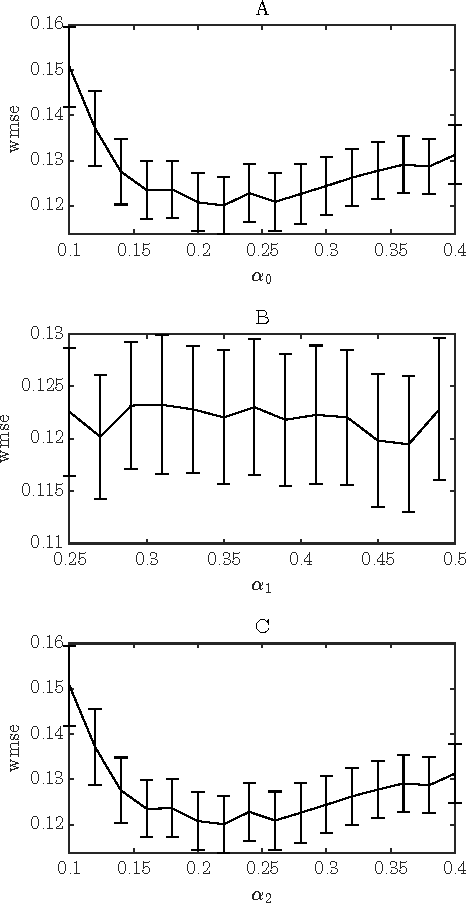
\includegraphics{hgParams.pdf}
        \caption[Non-parametric comparison]{Comparison of different parametric algorithms with standard deviations represented as error bars.}
        \label{fig:paramHg}
    \end{center}
\end{figure}

The use of curve fitting has, up until now been avoided. This is due to the difficulty in procuring the forms of these curves. Take Figure~\ref{fig:RODTestSet} where the first iteration produces no significant change. By fitting a curve, the results here could be misrepresented, so interpolation has been used in most cases to guide the eye. In Figure~\ref{fig:paramHg}, it was considered essential to present the different in form between ${\alpha_0}$, ${\alpha_1}$, and ${\alpha_2}$ so a curve has been added to guide the reader to the differences in form. Polynomial fits were used for each subfigure, with A and B using 1st order and C using 4th order.

\section{Problem Sensitivity}
The problem set up provides an estimation of a fixed number of iteration and sample size. What if these change? Are the parameters overfitted to this specific problem? If deviations from this are taken, are the intelligent methods worse than Monte Carlo? This is important to determine, as there is a significant potential cost to such an inefficiency.

Monte Carlo is tested compared to RoDGer and RoD, using the already fitted parameters where required. Monte Carlo is included to demonstrate the baseline case, while RoDGer is included due to producing the best results in previous testing. RoD has been included to assess if the learning rate maintains significantly higher than Monte Carlo in an extended testing range. Results have been presented in Figure~\ref{fig:sensi1}. Convergence of RoD to Monte Carlo is observed, with RoDGer consistently outperforming the other two algorithms.

\begin{figure}[H]
    \begin{center}
        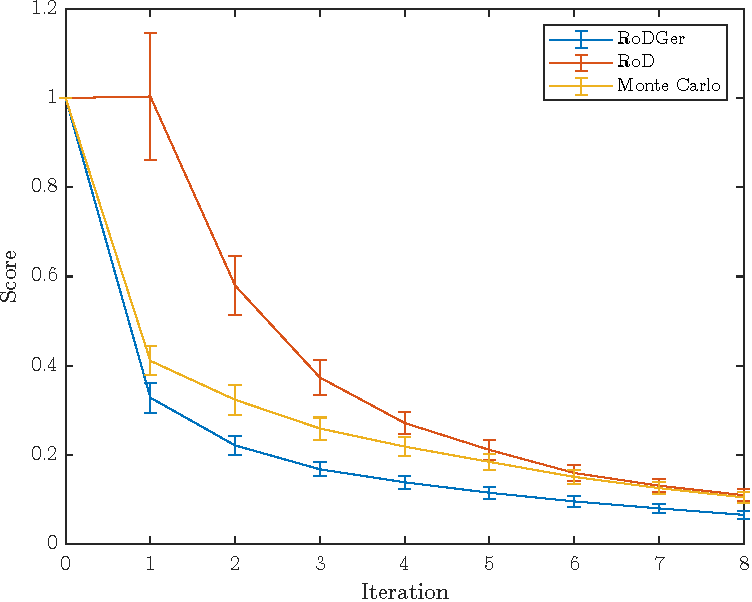
\includegraphics{Sensi1.pdf}
        \caption[Results of prolonged sampling]{Comparison of different parametric algorithms with standard deviations represented as error bars over an extended number of iterations.}
        \label{fig:sensi1}
    \end{center}
\end{figure}

Using sample sizes of 50 and 150 on Monte Carlo and RoDGer supports the power of RoDGer over simply using Monte  Carlo.

\begin{figure}[H]
    \begin{center}
        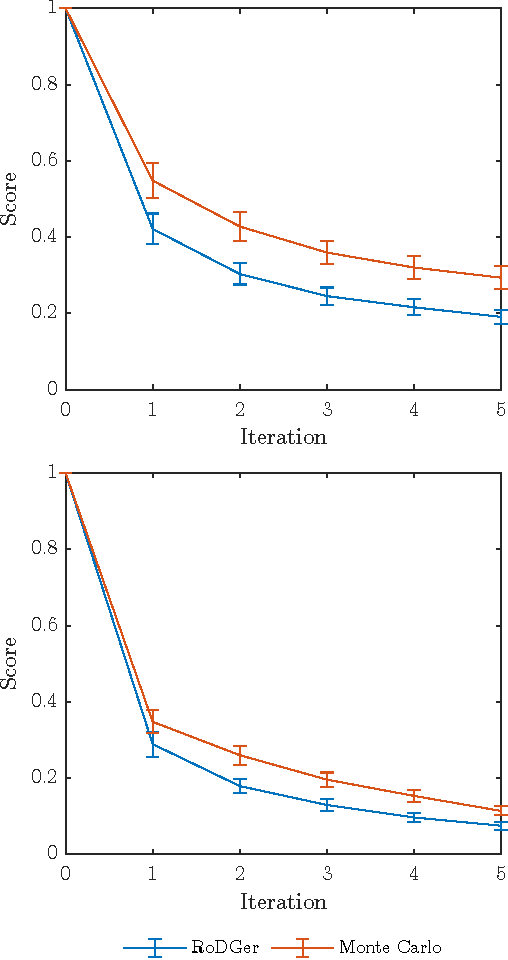
\includegraphics{Sensi2.pdf}
        \caption[Results of prolonged sampling]{Comparison of different parametric algorithms with standard deviations represented as error bars over an extended number of iterations.}
        \label{fig:sensi2}
    \end{center}
\end{figure}


\section{Refinement}
There are several points for progression that are worth discussing. Firstly, the training system requires improvement. Despite the observations of parallelisation leading to a situation of $\mathcal{O}(c)$ given an infinite number of processing units, an infinite number of processing units unfortunately do not exist. In the event of three parameters, the current methodology requires $N_\mathrm{train}\prod(n_{\alpha_i})$ executions of the learning algorithm, where $n_{\alpha_i}$ is the number of different values tested for $\alpha_i$. Even with simply 3 different values tested for each parameter in the Holy Trinity algorithm, this equates to $\sim{}4500$ executions of the algorithm. Thus, as the maximum number of CPUs available was 380, the training process became $\mathcal{O}\left(N_\mathrm{train}\prod{n_{\alpha_i}}\right)$. A potential solution would be segmentation, where the datasets are split into smaller groups with which are tested on a sample of the parameter space, with results from these smaller groups amalgamated at the end. Additionally, active learning could be used in the determination of the minima. Here, the goal would be to find the minima using as few parameter values as possible.

The current implementation of the scoring system is simple. Although this would please Occam's barber, it is believed that this is not satisfactory for the aggressive pursuit of effective drugs. One possibility is only scoring samples which show a pChEMBL greater than seven. This puts a greater weight on these samples, although a multidisciplinary discussion is required here. This could potentially be aided by categorising the data set instead, instead separating results into $\mathrm{pChEMBL}>7$ and $\mathrm{pChEMBL}\leq{}7$.

\section{Link to Covid}
\blindtext[1]


%!TEX root = ../thesis.tex
%*******************************************************************************
%****************************** Third Chapter **********************************
%*******************************************************************************
\chapter{Conclusion}

% **************************** Define Graphics Path **************************

\graphicspath{{Chapter6/Figs/Vector/}{Chapter6/Figs/}}




There are about 20000 drugs approved for pharmaceutical use, with more being trialled every year. However, there is hesitancy in using these drugs as treatments for emerging diseases. Instead, focus is given to designer drugs which may take years to develop. It is estimated 80\% of the cost in drug design and manufacture arises simply from the developing process. This was shown to be ineffective at the time of the SARS-CoV-2 outbreak whereby the use of existing drugs was slow, and often polluted with misinformation.

In order to combat these issues, the role of active learning cannot be understated. Reviewing drugs with low manufacturing costs as treatments for incurable diseases.
%\include{Chapter7/chapter7}

% ********************************** Back Matter *******************************
% Backmatter should be commented out, if you are using appendices after References
%\backmatter

% ********************************** Bibliography ******************************
\begin{spacing}{0.9}

    % To use the conventional natbib style referencing
    % Bibliography style previews: http://nodonn.tipido.net/bibstyle.php
    % Reference styles: http://sites.stat.psu.edu/~surajit/present/bib.htm

    % \bibliographystyle{apalike}
    %\bibliographystyle{unsrt} % Use for unsorted references  
    %\bibliographystyle{plainnat} % use this to have URLs listed in References
    % \cleardoublepage
    % \bibliography{References/references} % Path to your References.bib file


    % If you would like to use BibLaTeX for your references, pass `custombib' as
    % an option in the document class. The location of 'reference.bib' should be
    % specified in the preamble.tex file in the custombib section.
    % Comment out the lines related to natbib above and uncomment the following line.

    \printbibliography[heading=bibintoc, title={References}]{}


\end{spacing}

% ********************************** Appendices ********************************

% \begin{appendices} % Using appendices environment for more functionality

%     %!TEX root = ../thesis.tex
% ******************************* Thesis Appendix A ****************************

%     %!TEX root = ../thesis.tex
% ******************************* Thesis Appendix B ********************************


% \end{appendices}

% *************************************** Index ********************************
% \printthesisindex % If index is present

\end{document}